\documentclass[sigconf,nonacm]{acmart}

\usepackage{booktabs}
\usepackage{graphicx}
\usepackage{multirow}
\sloppy

\settopmatter{printacmref=false}
\renewcommand\footnotetextcopyrightpermission[1]{}
\pagestyle{plain}

\begin{document}

\title{Role-Unit: Fitness-Guided Model Assignment for Cost-Efficient Multi-Agent LLM Systems}

\author{Ahasan Kabir}
\affiliation{%
  \institution{University of Central Florida}
  \city{Orlando}
  \state{Florida}
  \country{USA}
}
\email{ahasan.kabir@ucf.edu}

\begin{abstract}
Multi-agent LLM systems assign specialized roles to language models, yet selecting which model serves each role is typically done ad hoc. We propose \textit{Role-Unit}, a framework that unit-tests each candidate model on role-specific tasks using a held-out validation set, then formulates the assignment as a budget-constrained Integer Linear Program (ILP) to jointly optimize accuracy and cost. We evaluate on MMLU across three domain roles (Historian, Scientist, Economist) with six open-weight models (3B--24B parameters). Our ILP-optimal assignments produce a Pareto frontier that dominates both homogeneous (single-model) and random baselines at every cost level. At the balanced operating point, Role-Unit achieves 82.6\% accuracy at 36\% lower cost than the best homogeneous baseline, demonstrating that lightweight fitness testing enables principled, cost-efficient model-to-role assignment.
\end{abstract}

\maketitle

\section{Introduction}

Multi-agent systems built on large language models (LLMs) assign functional roles---such as domain expert, critic, or aggregator---to individual models~\cite{guo2024large, qian2024chatdev}. A recurring challenge is \textit{model assignment}: deciding which LLM should fill each role. In practice, teams default to using the same strong model everywhere (homogeneous deployment) or make ad-hoc choices, leaving potential accuracy and cost gains unexplored.

This problem is non-trivial because models exhibit uneven strengths across domains. A model that excels at scientific reasoning may underperform on economics, and the most accurate model is often the most expensive. As model pools grow and roles multiply, the assignment space becomes combinatorial ($M^R$ possibilities for $M$ models and $R$ roles), ruling out manual search.

We introduce \textbf{Role-Unit}, a two-stage framework: (1)~\textit{fitness testing}---evaluate every candidate model on each role's domain tasks using a validation split, producing a fitness matrix and an empirical cost matrix; (2)~\textit{ILP-optimal assignment}---formulate model selection as a Multiple-Choice Knapsack Problem (MCKP) and solve it with Integer Linear Programming, sweeping budget levels to produce a Pareto frontier of accuracy--cost tradeoffs.

Our contributions are: (i) a systematic unit-testing protocol for measuring per-role model fitness; (ii) an ILP formulation that jointly optimizes accuracy and inference cost; and (iii) empirical validation on MMLU with six open-weight models showing that fitness-guided assignment consistently outperforms baselines.

\section{Related Work}

\textbf{Multi-agent LLM systems.} Recent work coordinates multiple LLM agents for complex tasks. Du et al.~\cite{du2024improving} show that multi-agent debate improves factuality. ChatDev~\cite{qian2024chatdev} assigns software engineering roles (programmer, reviewer) to LLM agents in a structured pipeline. Guo et al.~\cite{guo2024large} survey the space, identifying agent profiling and topology as key design axes. These systems fix role--model mappings without systematic evaluation.

\textbf{LLM routing and model selection.} Hybrid LLM~\cite{ding2024hybrid} routes queries to small or large models based on predicted difficulty. RouteLLM~\cite{ong2024routellm} trains routers from human preference data for cost-quality tradeoffs. MasRouter~\cite{zhong2025masrouter} addresses multi-agent routing via a learned controller. Unlike these approaches, Role-Unit requires no training---fitness scores are computed directly from validation performance.

\textbf{Role-playing and expert personas.} ExpertPrompting~\cite{xu2023expertprompting} generates domain expert personas to improve LLM response quality. We adopt role-specific system prompts similarly but focus on \textit{evaluating} which model best fits each role, rather than prompt design.

\textbf{Benchmarking.} We build on MMLU~\cite{hendrycks2021measuring}, a 57-subject multiple-choice benchmark. We map 23 domain-specific subjects to three expert roles, creating a structured evaluation for role--model fitness.

\section{Methodology}

\subsection{Problem Formulation}

Given $M$ candidate models and $R$ domain roles, let $f_{m,r}$ denote the fitness (accuracy) of model~$m$ on role~$r$, and $c_{m,r}$ the inference cost. We seek an assignment $A: \text{roles} \rightarrow \text{models}$ that maximizes accuracy within a cost budget~$B$:
\begin{equation}
\max_{x} \sum_{r} w_r \sum_{m} x_{m,r} \cdot f_{m,r}
\label{eq:obj}
\end{equation}
subject to: $\sum_{m} x_{m,r} = 1\ \forall r$ (one model per role), $\sum_{r,m} x_{m,r} \cdot c_{m,r} \leq B$ (budget), and $x_{m,r} \in \{0,1\}$. Here $w_r$ is the proportion of questions for role $r$. This is a Multiple-Choice Knapsack Problem, solvable optimally via standard ILP solvers.

\subsection{Fitness Testing (Stage 1)}

We evaluate all $M \times R$ model--role combinations on the MMLU validation split. Each question is routed to its domain role (based on subject--role mapping) and answered by the assigned model using a role-specific system prompt. We record accuracy, token usage, and cost per (model, role) pair, producing the fitness matrix $\mathbf{F}$ and cost matrix $\mathbf{C}$.

\subsection{ILP Assignment (Stage 2)}

We sweep budget $B$ from the minimum possible cost (cheapest model per role) to the maximum (most expensive), solving the ILP at each level. The set of non-dominated solutions forms the Pareto frontier. We use the CBC solver via PuLP.

\subsection{Experimental Setup}

\textbf{Models}: Six open-weight models served via vLLM on two NVIDIA B200 GPUs: Mistral-Small-24B, Qwen2.5-Coder-14B, Gemma-2-9B, Llama-3.1-8B, Qwen2.5-7B, and Llama-3.2-3B.

\textbf{Roles}: Three domain roles (Historian, Scientist, Economist) covering 23 MMLU subjects. Each role has a domain-specific system prompt.

\textbf{Data}: Validation split (477 questions) for fitness testing; test split (488 stratified-sampled questions) for baseline evaluation.

\textbf{Cost}: OpenRouter-equivalent pricing per model, computed from actual token usage during validation.

\textbf{Baselines}: (1) Homogeneous---same model for all roles (6 configurations); (2) Random---random model per role (5 trials, seed 42).

\section{Preliminary Results}

\begin{table}[t]
\caption{Validation fitness matrix: accuracy per (model, role). Bold indicates best per role.}
\label{tab:fitness}
\centering
\small
\begin{tabular}{lcccc}
\toprule
Model & Hist. & Sci. & Econ. & Mean \\
\midrule
Mistral-24B & \textbf{.902} & \textbf{.806} & \textbf{.866} & \textbf{.858} \\
Gemma-9B & .851 & .670 & .821 & .781 \\
Qwen-7B & .833 & .660 & .714 & .736 \\
Qwen-Coder-14B & .833 & .623 & .732 & .730 \\
Llama-8B & .816 & .681 & .571 & .689 \\
Llama-3B & .770 & .565 & .464 & .600 \\
\bottomrule
\end{tabular}
\end{table}

\begin{table}[t]
\caption{Strategy comparison. ILP points are from the Pareto frontier (validation). Baselines are evaluated on the test split (488 questions).}
\label{tab:comparison}
\centering
\small
\begin{tabular}{lcc}
\toprule
Strategy & Accuracy & Cost (\textcent) \\
\midrule
\textit{ILP-Optimal (Pareto):} & & \\
\quad P7: Balanced & .826 & 0.93 \\
\quad P4: Efficient & .776 & 0.64 \\
\quad P10: Max Accuracy & .855 & 1.46 \\
\midrule
\textit{Homogeneous (test):} & & \\
\quad Mistral-24B (best) & .820 & 1.46 \\
\quad Gemma-9B (\#2) & .775 & 0.82 \\
\quad Llama-3B (cheapest) & .646 & 0.36 \\
\midrule
\textit{Random (test):} & & \\
\quad Mean $\pm$ std (5 trials) & .727 $\pm$ .036 & 0.93 \\
\bottomrule
\end{tabular}
\end{table}

Table~\ref{tab:fitness} shows the validation fitness matrix. Mistral-24B leads all roles, but Gemma-9B is competitive on Historian and Economist at roughly half the cost. Scientist is the hardest role across all models, with accuracy 10--20 points lower than Historian.

Table~\ref{tab:comparison} compares strategies. The ILP balanced point (P7: Gemma for Historian and Economist, Mistral for Scientist) achieves 82.6\% accuracy at 0.93\textcent---matching the best homogeneous baseline's accuracy (82.0\%) while costing 36\% less. The efficient point (P4) reaches 77.6\% at only 0.64\textcent, comparable to Gemma homogeneous (77.5\%) at 22\% lower cost.

\begin{figure}[t]
\centering
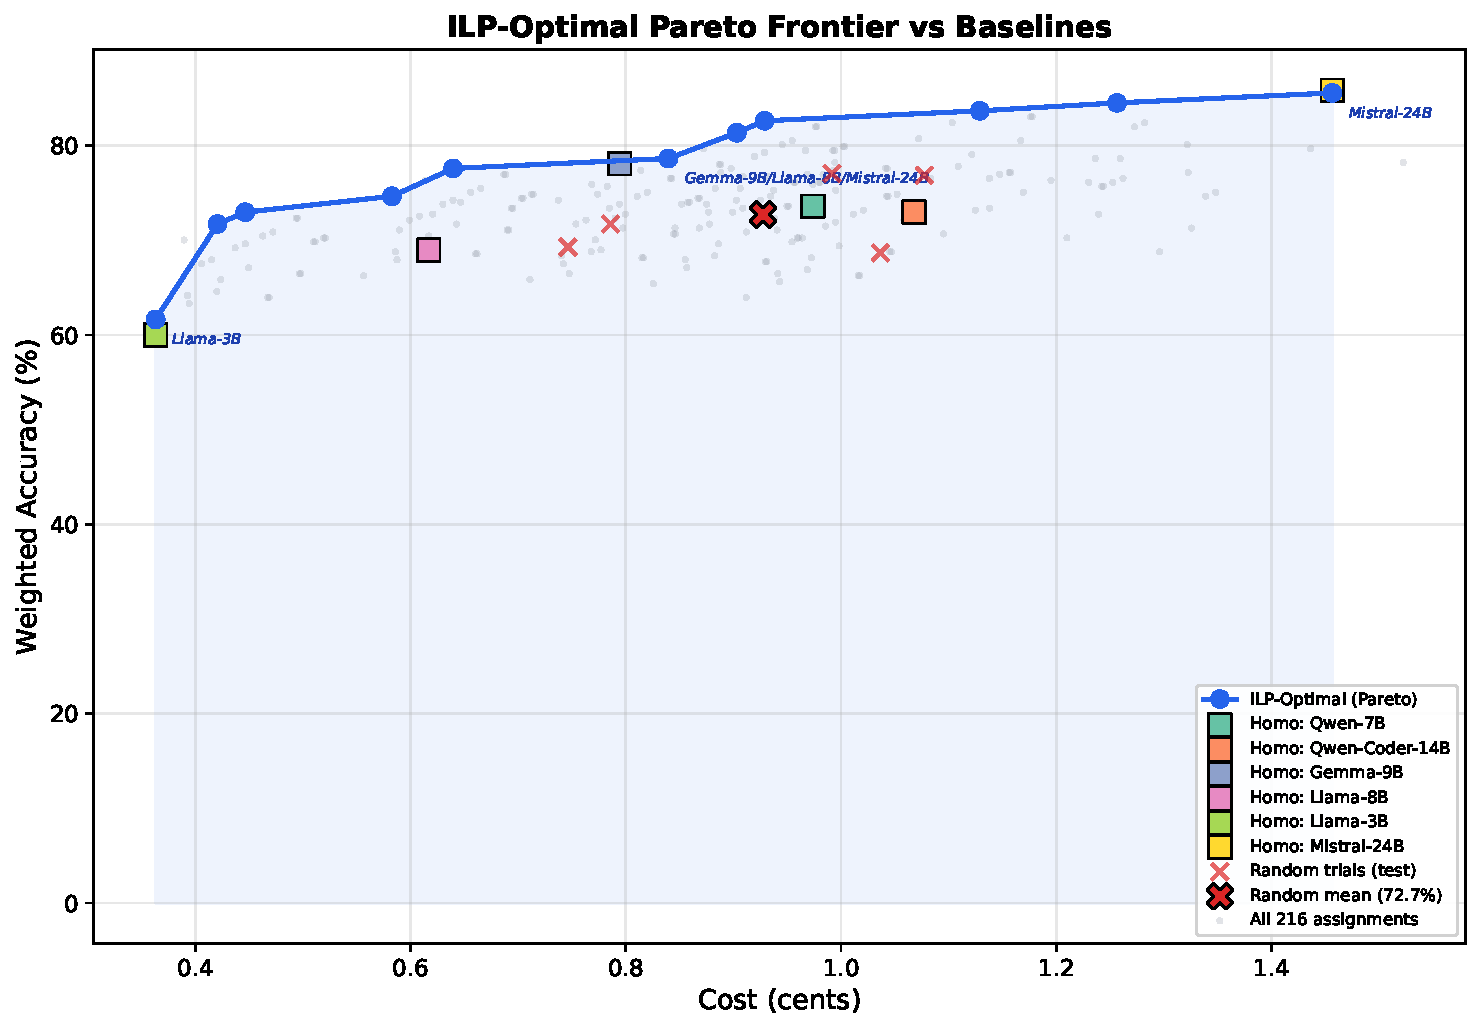
\includegraphics[width=\columnwidth,alt={Pareto frontier plot showing ILP-optimal assignments dominating baselines across all cost levels}]{figures/pareto_frontier.pdf}
\caption{ILP-optimal Pareto frontier (blue line) vs.\ all 216 possible assignments (gray), homogeneous baselines (colored squares), and random trials (red). Every Pareto point dominates or matches the baselines at its cost level.}
\label{fig:pareto}
\end{figure}

Figure~\ref{fig:pareto} visualizes the Pareto frontier. The ILP curve (blue) sits at or above every baseline at each cost level. Key insight: the optimizer identifies that Gemma-9B is nearly as strong as Mistral-24B on Historian/Economist but much cheaper, so it allocates budget to Mistral only for Scientist---the hardest role where the accuracy gap is largest (80.6\% vs.\ 67.0\%).

Random assignment averages 72.7\% accuracy at 0.93\textcent, underperforming both the ILP balanced point (+9.9 points at equal cost) and the cheapest ILP point P1 (71.7\% at 0.42\textcent---less than half the cost).

\textbf{Next steps.} We plan to: (1) evaluate the ILP-selected assignments on the full MMLU test split; (2) extend to cognitive roles (Critic, Reflector) and multi-step debate topologies; (3) explore scaling to larger model pools where ILP solver efficiency becomes critical.

\bibliographystyle{ACM-Reference-Format}
\begin{thebibliography}{8}
\small

\bibitem{du2024improving}
Y.~Du, S.~Li, A.~Torralba, J.~B.~Tenenbaum, and I.~Mordatch. 2024. Improving factuality and reasoning in language models through multiagent debate. In \textit{Proc.\ ICML}. JMLR.org.

\bibitem{guo2024large}
T.~Guo, X.~Chen, Y.~Wang, R.~Chang, S.~Pei, N.~V.~Chawla, O.~Wiest, and X.~Zhang. 2024. Large language model based multi-agents: A survey of progress and challenges. In \textit{Proc.\ IJCAI}, 8048--8057.

\bibitem{qian2024chatdev}
C.~Qian, W.~Liu, H.~Liu, N.~Chen, et~al. 2024. ChatDev: Communicative agents for software development. In \textit{Proc.\ ACL}, 15174--15186.

\bibitem{ding2024hybrid}
D.~Ding, A.~Mallick, C.~Wang, R.~Sim, S.~Mukherjee, V.~R\"{u}hle, L.~V.~S.~Lakshmanan, and A.~H.~Awadallah. 2024. Hybrid LLM: Cost-efficient and quality-aware query routing. In \textit{Proc.\ ICLR}.

\bibitem{ong2024routellm}
I.~Ong, A.~Almahairi, V.~Wu, W.-L.~Chiang, T.~Wu, J.~E.~Gonzalez, M.~W.~Kadous, and I.~Stoica. 2024. RouteLLM: Learning to route LLMs with preference data. \textit{arXiv:2406.18665}.

\bibitem{zhong2025masrouter}
Zhong et~al. 2025. MasRouter: Learning to route LLMs for multi-agent systems. \textit{arXiv:2502.11133}.

\bibitem{xu2023expertprompting}
B.~Xu, A.~Yang, J.~Lin, Q.~Wang, C.~Zhou, Y.~Zhang, and Z.~Mao. 2023. ExpertPrompting: Instructing large language models to be distinguished experts. \textit{arXiv:2305.14688}.

\bibitem{hendrycks2021measuring}
D.~Hendrycks, C.~Burns, S.~Basart, A.~Zou, M.~Mazeika, D.~Song, and J.~Steinhardt. 2021. Measuring massive multitask language understanding. In \textit{Proc.\ ICLR}.

\end{thebibliography}

\end{document}
